\subsection{\textit{Modeling} dan Validasi}
\label{subsec:knn-validasi}

\subsubsection{Skema Validasi}
Setelah deduplikasi, sebanyak 27.309 baris dibagi secara \textit{stratified} dengan \textit{seed} 42 menjadi \textbf{21.847 data development} (80\%) dan \textbf{5.462 data holdout} (20\%). Seluruh pemilihan fitur dan hiperparameter dilakukan pada development. Data \textit{holdout} baru digunakan setelah konfigurasi ditentukan untuk memperoleh evaluasi yang terpisah dari proses pemilihan model.

Pada development, sepuluh kandidat fitur terlebih dahulu dibandingkan dengan \textit{stratified} 3-\textit{fold} CV. Dua representasi dengan Macro F1 tertinggi kemudian diuji dengan \textit{stratified} 5-\textit{fold} CV untuk mencari hiperparameter. Dalam setiap \textit{fold}, imputasi, normalisasi, dan kategori \textit{one-hot} di-\textit{fit} pada bagian latih saja. Nilai evaluasi yang dilaporkan adalah rata-rata Macro F1 tiap \textit{fold} beserta simpangan baku sampelnya. Skema ini menghindari kebocoran statistik \textit{preprocessing} dari \textit{fold} validasi, namun pemilihan dua kandidat awal dan pencarian parameter memakai development yang sama sehingga skor CV terbaik tetap merupakan hasil pemilihan model.

\subsubsection{\textit{Hyperparameter Tuning}}
Pencarian dilakukan atas dua representasi fitur, tujuh pilihan $k$, dan tiga metrik jarak. Total terdapat \textbf{42 konfigurasi}, semuanya menggunakan suara mayoritas tanpa pembobotan jarak. Ruang pencarian ditampilkan pada Tabel~\ref{tab:knn-grid}.

\begin{table}[H]
 \centering
 \caption{Ruang pencarian hiperparameter KNN}
 \label{tab:knn-grid}
 \begin{tabularx}{\textwidth}{l Y l}
  \toprule
  \textbf{Komponen} & \textbf{Kandidat} & \textbf{Terpilih} \\
  \midrule
  Representasi & 16 atau 15 fitur hasil seleksi & 16 fitur \\
  $k$ & 3, 5, 7, 9, 11, 15, 21 & 7 \\
  Metrik jarak & Manhattan, Euclidean, Minkowski ($p=3$) & Manhattan \\
  Pembobotan suara & \textit{Uniform} (tetap) & \textit{Uniform} \\
  \bottomrule
 \end{tabularx}
\end{table}

Hasil terbaik untuk setiap pasangan representasi dan metrik ditampilkan pada Tabel~\ref{tab:knn-tuning}. Nilai dalam tabel berasal dari berkas \nolinkurl{output/knn/tuning.csv}. Pada kombinasi yang diuji, konfigurasi 16 fitur dengan Manhattan $k=7$ memberikan rata-rata Macro F1 tertinggi, yaitu 0,82126.

\begin{table}[H]
 \centering
 \caption{Konfigurasi terbaik per representasi dan metrik pada 5-\textit{fold} CV}
 \label{tab:knn-tuning}
 \begin{tabular}{c l c c c}
  \toprule
  \textbf{Fitur} & \textbf{Jarak} & $\boldsymbol{k}$ & \textbf{Macro F1} & \textbf{SD} \\
  \midrule
  16 & Manhattan & 7 & \textbf{0,82126} & 0,00714 \\
  16 & Minkowski ($p=3$) & 7 & 0,82040 & 0,00721 \\
  16 & Euclidean & 7 & 0,82015 & 0,00724 \\
  15 & Minkowski ($p=3$) & 7 & 0,82013 & 0,00671 \\
  15 & Manhattan & 5 & 0,81955 & 0,00663 \\
  15 & Euclidean & 7 & 0,81869 & 0,00669 \\
  \bottomrule
 \end{tabular}
\end{table}

\begin{figure}[H]
 \centering
 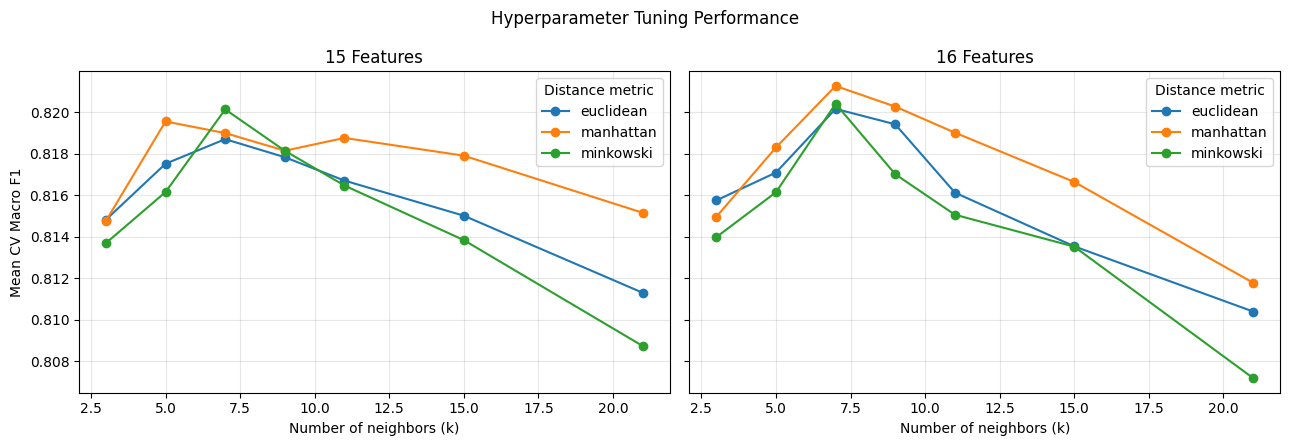
\includegraphics[width=0.94\textwidth]{knn/knn_tuning.png}
 \caption{Rata-rata Macro F1 validasi silang menurut $k$ dan metrik jarak pada dua representasi fitur}
 \label{fig:knn-tuning}
\end{figure}

Gambar~\ref{fig:knn-tuning} menunjukkan bahwa kinerja berubah ketika jumlah tetangga atau metrik jarak diganti. Perbedaan antar konfigurasi terbaik relatif kecil, yaitu 0,00086 antara Manhattan dan Minkowski pada 16 fitur. Nilai ini juga lebih kecil daripada simpangan baku antar-\textit{fold} sekitar 0,007. Oleh sebab itu, konfigurasi terbaik dipahami sebagai pilihan berdasarkan rata-rata pada ruang pencarian yang diuji, bukan bukti keunggulan yang pasti untuk semua pembagian data.

\subsubsection{Model Final}
KNN final menggunakan \textbf{16 fitur, Manhattan, $k=7$, dan suara mayoritas uniform}. Skor development CV adalah $\text{Macro F1}=0{,}82126\pm0{,}00714$, dengan \textit{accuracy} rata-rata 0,84552. Kelima skor Macro F1 per \textit{fold} adalah 0,82781, 0,81894, 0,81019, 0,82685, dan 0,82251. Model kemudian di-\textit{fit} pada seluruh development dan dievaluasi sekali pada \textit{holdout}, sebagaimana dibahas pada Subbab~\ref{subsec:knn-hasil}.

Untuk membuat prediksi data uji, konfigurasi yang sama di-\textit{fit} ulang pada \textbf{27.309 data latih bersih}. Pipeline menyimpan model dan statistik \textit{preprocessing} di \nolinkurl{output/knn/model.pkl}, hasil pencarian di \nolinkurl{output/knn/tuning.csv}, dan prediksi \textbf{6.844 baris} di \nolinkurl{output/knn/submission.csv}. Artefak tersebut dapat direproduksi melalui \nolinkurl{src/kaggle/knn_notebook.ipynb} atau \nolinkurl{src/kaggle/knn_submission.py}.